\begin{frame}{Характиристики плёнки, теплообмен между твёрдым веществом и жидкостью, скорость испарения жидкости.}
\begin{block}{\sl Проводимоть в паровом зазоре - основоной механизм теплообмена между твёрдым и жидким}
Тепловой поток на единицу площади  \(k\frac{T_{S}-T_{B}}{b} = \frac{k\triangle T}{b}\), где \(\triangle T\) - разница температур между твёрдым веществом и температурой кимения жидкости k - теплопроводность пара.
\end{block}
Введём массу жидкости испаряющуюся за единицу времени \(\dot{M}\) после короткого времени, для возвращения значения температуры до \(T_{B}\), понадобится \(L\dot{M}\sim\left(\frac{k\triangle T}{b}\right)R^{2}\), L - теплота парообразования. Осталось определить b - толщину плёнки и \(\dot{M}\). Из рисунка ({b}) видно, что зазор (паровой слой) имеет размеры: несколько миллиметров в длине и 0,1 мм в толщине. Поэтому пар выходит с течением Пуазейля.
\end{frame}

\begin{frame}{}
\center{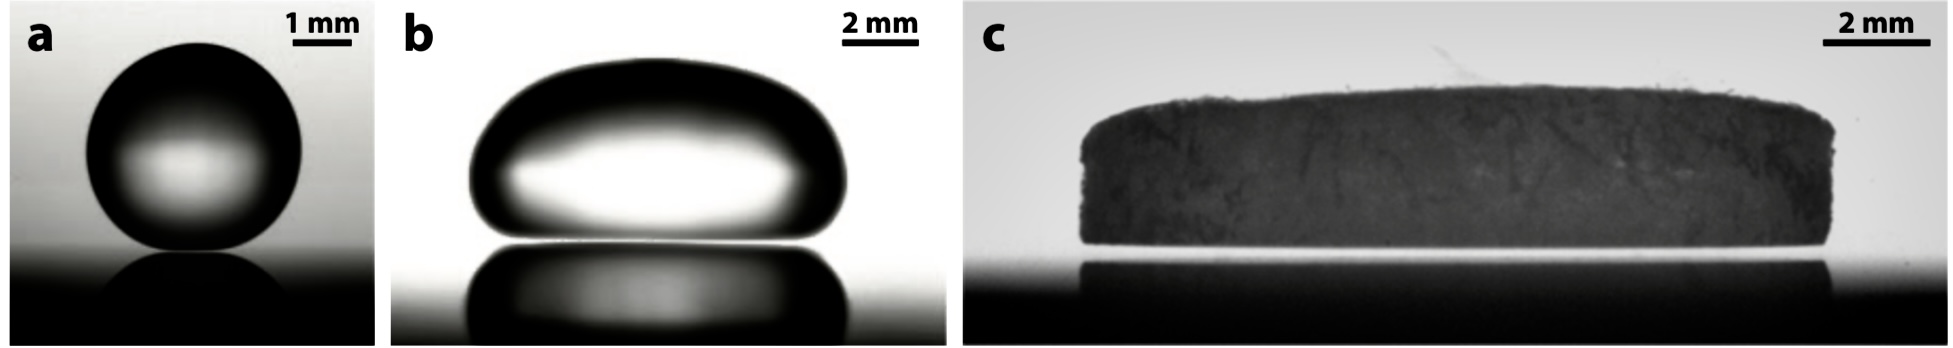
\includegraphics[width=\linewidth]{foto/IMG_7591.jpg}}
\begin{block}{\slВведём зависимость между потоком пара и градиетом давления:}
\(\dot{M}\sim\left(\frac{\rho_{\upsilon}Rb^{3}}{\eta_{\upsilon}}\right)\triangledown P\), где \(\rho_{\upsilon} и \eta_{\upsilon}\) - плотноть пара и вязкость, капля оказывает гидростатическое давление \(\rho g\iota_{c}\), откуда \(\dot{M}\sim\left(\frac{\rho_{\upsilon}b^{3}}{\eta_{\upsilon}}\right)\rho g\iota_{c}\), в стационарном режиме плёнка питается испарением капли со скоростью, с которой пар ускользает, что даёт закон для толщины плёнки \(b\sim\left(R\beta\right)^{1/2}\), где \(\beta = {\left(\frac{k\triangle T\eta_{\upsilon}}{L\rhoa_{\upsilon}\rhoa g\iota_{c}}\right)}^{1/2}\), подсчитав значения для b и подставляя их в формулу для \(\dot{M}\) мы получим значение пара, образованного в единицу времени.
\end{block}
\end{frame}

\begin{frame}{}
\begin{block}{\sl Итог:}
Предполагая, что капля испаряется только своим дном получим время жизни капель Лейденфроста: \(\tau=\frac{M}{\dot{M}}\). Если счиать, что время жизни мало, то формуля для теплопроводности будет упрощена и иметь вид: \( \dot{M} \sim \left(\frac{k \triangle T}{Lb}\right)R^{2} \sim \rho_{\upsilon}\dot{b}R^{2}\), в предположении что b должен зависить от времени как: \(\left(\frac{k\triangle Tt}{L\rho_{\upsilon}}\right)^{1/2}\)
\end{block}
\center{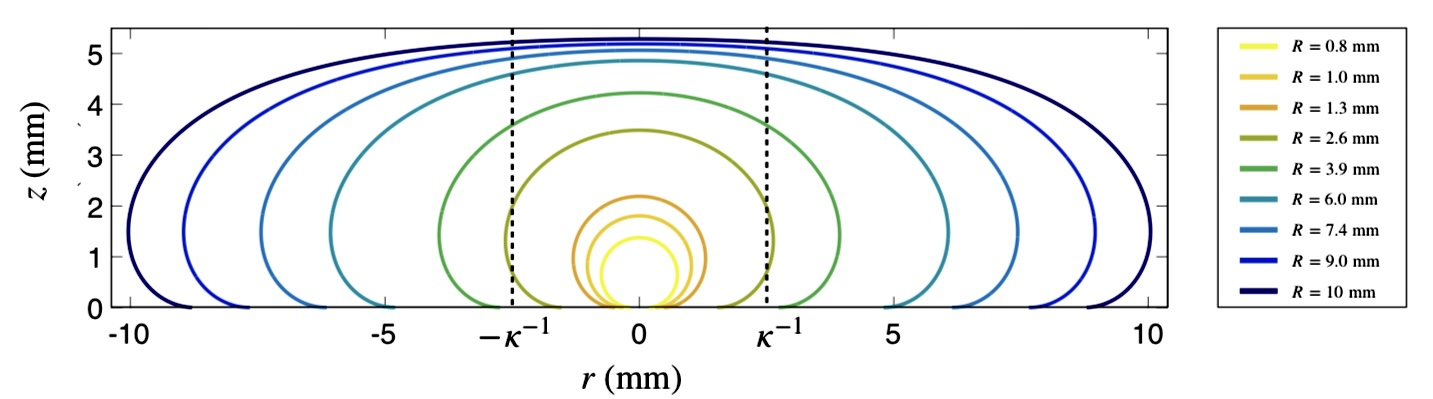
\includegraphics[width=\linewidth]{IMG_7597.jpg}}
\end{frame}

\begin{frame}{Установка}
\sidefig (0.5\linewidth)(0.5\linewidth) {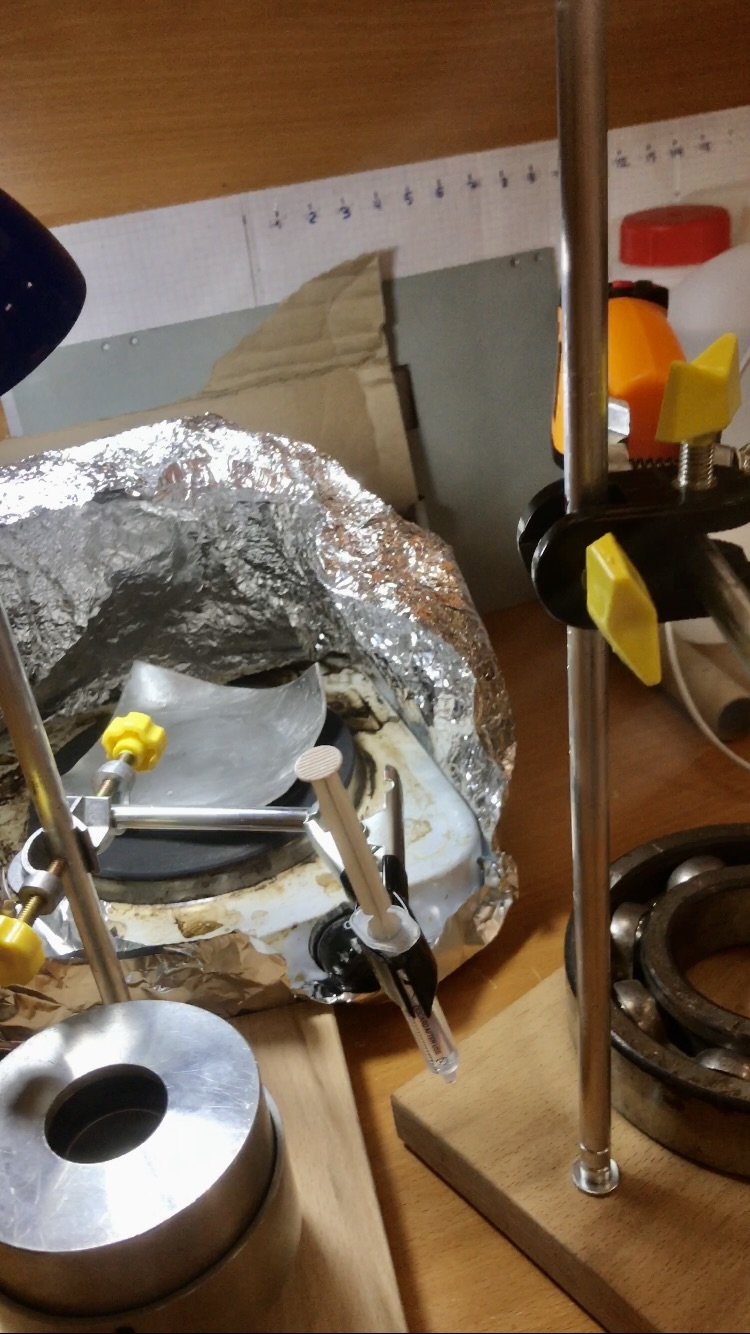
\includegraphics[scale=0.155]{97B356EC-468F-416D-9B06-919921896A27_1_201_a.jpeg}}{В установке пришлось использовать \textcolor[RGB]{0,128,255}{\sl два штатива}, для фиксации \textcolor[RGB]{0,128,255}{\sl лазерного термометра и шприца с дистилированой водой}, с целью не изменять их наклон и высоту во воремя эксперемента, а так же, чтобы изолировать систему от ветра и конвекционных потоков, использовали \textcolor[RGB]{0,128,255}{\sl защитную конструкцию из фальги}. Нагревали, \textcolor[RGB]{0,128,255}{\sl отшлифованную алюминиевую пластину}, в которой сделали углубления для удержания капли на месте.}

\end{frame}

\begin{frame}{}
\sidefig (0.5\linewidth)(0.5\linewidth)
{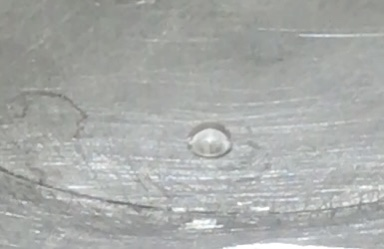
\includegraphics[scale=0.35]{5F8D7E02-0952-4090-83E1-37FAFF303F95_4_5005_c.jpeg}}{\vspace{0.10cm}Измерение проводились в пределах от 220\(C^{\circ}\) до 50 \(C^{\circ}\). Капали с помощью щприца, для чего провели предварительное измерение капель, с помощью весов, добившись одинаковые значения для масс капель, настроив установку, получили среднее}
\sidefig (0.5\linewidth)(0.5\linewidth)
{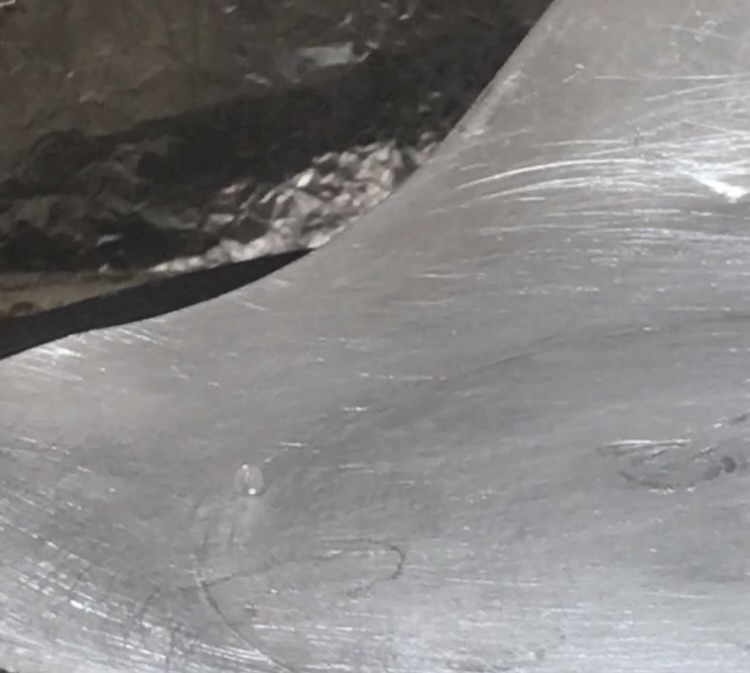
\includegraphics[scale=0.18]{A82B7535-E316-43B4-BE76-A6D4F11E907F_1_201_a.jpeg}}{значения для массы капли:\\
\[\overline{M} = 0,042 \pm 0,001 g. \]
Шприц, мы отворачивали и поворачивали обратно, чтобы избежать нагрева воды, так как капать необходимо было с минимальной высоты}
\end{frame}